\documentclass[theme=teal]{khmermath}
\usepackage{needspace}

\geometry{left=0.85cm, right=0.85cm, top=0.75cm, bottom=1.35cm, footskip=0.65cm}
\usepackage{colortbl}
\usepackage{tikz}
\usetikzlibrary{calc,shapes,arrows,intersections,through,backgrounds,shadows,decorations.pathmorphing,angles,quotes}

% -------------------------------------------------------------------------
% Korean Math Textbook Style Color Palette & Macros
% -------------------------------------------------------------------------
\definecolor{koreaTeal}{RGB}{0, 150, 155}       % Primary Header Teal/Cyan
\definecolor{koreaDarkTeal}{RGB}{0, 105, 110}   % Dark Teal Accent
\definecolor{koreaBeige}{RGB}{247, 244, 237}     % Concept Sidebar Beige (#F7F4EE)
\definecolor{koreaBeigeBorder}{RGB}{225, 218, 205}
\definecolor{koreaOrange}{RGB}{235, 115, 30}     % Problem Number Orange
\definecolor{koreaBlue}{RGB}{35, 110, 190}      % Standard Blue
\definecolor{koreaPurple}{RGB}{125, 50, 160}    % Purple Accent
\definecolor{koreaNumber}{RGB}{115, 125, 135}   % Problem Number Gray
\definecolor{koreaYellow}{RGB}{255, 246, 175}   % Yellow Highlight Tint

\definecolor{brandNavy}{RGB}{0, 105, 110}
\definecolor{brandBlue}{RGB}{0, 150, 155}
\definecolor{brandLightBlue}{RGB}{247, 244, 237}
\definecolor{brandCrimson}{RGB}{195, 35, 60}
\definecolor{brandCoral}{RGB}{235, 80, 75}
\definecolor{brandGold}{RGB}{215, 130, 10}
\definecolor{brandGoldBg}{RGB}{255, 252, 242}
\definecolor{brandTeal}{RGB}{0, 150, 155}
\definecolor{brandTealBg}{RGB}{244, 252, 250}
\definecolor{subtleGray}{RGB}{246, 251, 249}
\definecolor{cardBorder}{RGB}{220, 212, 198}

% Custom Header & Footer setup (Korean Textbook Style)
\usepackage{fancyhdr}
\pagestyle{fancy}
\fancyhf{}
\renewcommand{\headrulewidth}{0pt}
\renewcommand{\footrule}{\color{koreaTeal!60}\hrule height 0.6pt\vspace{2.5pt}}

\fancyfoot[L]{%
  \fontsize{8.5}{8.5}\selectfont\kml \color{koreaNumber}\textbf{\thepage}\ \vline\ \color{koreaDarkTeal}\textbf{ចម្ងាយរវាងពីរចំណុចក្នុងប្លង់កូអរដោនេ}%
}
\fancyfoot[C]{%
  \fontsize{8.5}{8.5}\selectfont\kby \color{koreaDarkTeal}\textbf{\ding{72}\ រៀបរៀងដោយ ៖ \textcolor{koreaDarkTeal}{ក្រូត រស្មី}\ \ding{72}}%
}
\fancyfoot[R]{%
  \fontsize{8.5}{8.5}\selectfont\kby \color{koreaDarkTeal}\textbf{ក្លឹបសិក្សាគណិតវិទ្យា PCM}\ \vline\ \color{koreaNumber}\textbf{\thepage}%
}

% Korean Header Banner
\newcommand{\koreanheader}[2]{%
  \noindent%
  \begin{tikzpicture}[x=1cm, y=1cm]
    \fill[koreaTeal, rounded corners=12pt] (0, 0.1) -- (0, 0.95) -- (4.2, 0.95) [rounded corners=0pt] -- (4.8, 0.1) -- cycle;
    \node[white, font=\fontsize{11}{11}\selectfont\kml\bfseries] at (2.1, 0.52) {#1};
    \node[anchor=west, font=\fontsize{16}{16}\selectfont\kml\bfseries, color=koreaDarkTeal] at (4.9, 0.44) {#2};
    \node[anchor=east, font=\fontsize{8.5}{8.5}\selectfont\kby, color=gray!80] at (19.2, 0.48) {$>$ ក្លឹបសិក្សាគណិតវិទ្យា PCM};
  \end{tikzpicture}%
  \vspace{1pt}%
}

% Yellow Formula Highlight Box
\newcommand{\koreahl}[1]{\colorbox{koreaYellow}{\fontsize{8.5}{8.5}\selectfont\textbf{#1}}}

% General Rule Box (Teal/Navy Theme - ជាទូទៅ)
\newtcolorbox{khboxorange}[1][]{
  enhanced,
  colframe=brandNavy!40,
  colback=brandLightBlue,
  boxrule=0.7pt,
  arc=4.5pt,
  borderline west={3.5pt}{0pt}{brandNavy},
  drop fuzzy shadow=brandNavy!15,
  left=8pt, right=8pt, top=3.5pt, bottom=3pt,
  title={\fontsize{9}{9}\selectfont\kml\color{white}\ding{72}\ ជាទូទៅ },
  coltitle=white,
  colbacktitle=brandNavy,
  boxed title style={
    boxrule=0pt,
    arc=3.5pt,
    left=7pt, right=7pt, top=2pt, bottom=2pt
  },
  attach boxed title to top left={yshift*=-\tcboxedtitleheight/2, xshift=12pt},
  #1
}

% Practice Card Box
\newtcolorbox{khboxpractice}[1][]{
  enhanced,
  colframe=brandTeal,
  colback=brandTealBg,
  boxrule=0.75pt,
  arc=3.5pt,
  left=7pt, right=7pt, top=2.5pt, bottom=2.5pt,
  #1
}

% Example / Card Item Box
\newtcolorbox{khcard}[1][]{
  enhanced,
  colframe=cardBorder,
  colback=white,
  boxrule=0.65pt,
  arc=3.5pt,
  left=6pt, right=6pt, top=2.5pt, bottom=2.5pt,
  #1
}

% Section, Subsection & Header Badge Macros
\newcommand{\khsection}[2]{%
  \vspace{1pt}%
  \noindent%
  \begin{tikzpicture}
    \fill[rounded corners=5pt, brandNavy!7] (0,0) rectangle (19.3, 0.60);
    \fill[rounded corners=4pt, brandNavy] (0.05, 0.05) rectangle (0.55, 0.55);
    \node[white, font=\fontsize{9.5}{9.5}\selectfont\bfseries] at (0.30, 0.30) {#1};
    \fill[brandGold, rounded corners=1pt] (0.64, 0.12) rectangle (0.68, 0.48);
    \node[anchor=west, font=\fontsize{10.5}{10.5}\selectfont\kml, color=brandCrimson] at (0.74, 0.30) {\textbf{#2}};
  \end{tikzpicture}%
  \vspace{1pt}%
}

\def\splitnum#1#2{%
  \color{koreaNumber!65}#1\color{koreaOrange}#2%
}
\newcommand{\koreannum}[1]{%
  \ifstrempty{#1}{}{%
    \mbox{%
      \fontsize{18}{18}\selectfont\bfseries%
      \ifnum#1<10\relax%
        \color{koreaNumber!65}0\color{koreaOrange}#1%
      \else%
        \expandafter\splitnum#1%
      \fi%
    }\,\ %
  }%
}

% Khmer Sub-Question Badge
\newcommand{\khlabel}[1]{%
  \tikz[baseline=-0.6ex]{%
    \node[fill=brandCrimson, rounded corners=3pt, inner sep=1.8pt, minimum width=1.25em, minimum height=1.22em, text=white, font=\kml\fontsize{7.2}{7.2}\selectfont, align=center] (lbl) {\raisebox{0.2pt}{#1}};%
  }\,\ %
}
\newcommand{\exhead}[1]{\hangindent=24pt\hangafter=1\koreannum{#1}}

% Difficulty Badges
\newcommand{\badgebasic}{\tikz[baseline=-0.6ex]{\node[fill=brandBlue!15, text=brandBlue, draw=brandBlue!40, line width=0.4pt, rounded corners=2.5pt, inner sep=1.6pt, font=\fontsize{7}{7}\selectfont\kml] {គ្រឹះ};}\,\ }
\newcommand{\badgestandard}{\tikz[baseline=-0.6ex]{\node[fill=koreaOrange!15, text=koreaOrange, draw=koreaOrange!40, line width=0.4pt, rounded corners=2.5pt, inner sep=1.6pt, font=\fontsize{7}{7}\selectfont\kml] {មធ្យម};}\,\ }
\newcommand{\badgeadvanced}{\tikz[baseline=-0.6ex]{\node[fill=brandCrimson!15, text=brandCrimson, draw=brandCrimson!40, line width=0.4pt, rounded corners=2.5pt, inner sep=1.6pt, font=\fontsize{7}{7}\selectfont\kml] {ជឿនលឿន};}\,\ }
\newcommand{\badgesolution}{\tikz[baseline=-0.6ex]{\node[fill=koreaPurple!15, text=koreaPurple, draw=koreaPurple!40, line width=0.4pt, rounded corners=2.5pt, inner sep=1.6pt, font=\fontsize{7}{7}\selectfont\kml] {ស្រាយបញ្ជាក់};}\,\ }
\newcommand{\phead}[1]{\noindent\tikz[baseline=-0.6ex]{\node[fill=koreaDarkTeal, text=white, rounded corners=3pt, inner sep=2.2pt, font=\fontsize{8}{8}\selectfont\kml] {ប្រតិបត្តិ #1};}\,\ }

\setlength{\parindent}{0pt}
\setlength{\parskip}{1.2pt}
\setlength{\columnsep}{16pt}
\setlength{\columnseprule}{0.5pt}
\def\columnseprulecolor{\color{koreaTeal!40}}

\begin{document}

% =========================================================================
% PAGE 1: SECTION 1 (ចម្ងាយរវាងពីរចំណុច)
% =========================================================================
\koreanheader{មេរៀនទី៩}{ចម្ងាយរវាងពីរចំណុចក្នុងកូអរដោនេ}

\khsection{១}{ចម្ងាយរវាងពីរចំណុច (Distance Between Two Points)}

\begin{khboxorange}
  \begin{minipage}[c]{0.65\textwidth}
    \begin{itemize}[leftmargin=11pt, itemsep=1.5pt, topsep=0pt, parsep=0pt]
      \item[\color{brandNavy}\ding{228}] \textbf{គំនិតវិចារណញាណ  ៖}\\
      ចម្ងាយត្រង់រវាងពីរចំណុច $A(x_1, y_1)$ និង $B(x_2, y_2)$ គឺជា \textbf{អ៊ីប៉ូតេនុស} នៃត្រីកោណកែងមួយ ដែលមានជ្រុងដេកជាគម្លាតតាម $x$ ($|x_2 - x_1|$) និងជ្រុងឈរជាគម្លាតតាម $y$ ($|y_2 - y_1|$) ។
      \item[\color{brandCrimson}\ding{228}] \textbf{ការទាញរករូបមន្តតាមទ្រឹស្ដីបទពីតាគ័រ ៖}\\
      ក្នុងត្រីកោណកែង $ABC$ កែងត្រង់ $C(x_2, y_1)$ ៖
      \vspace{-2pt}
      \begin{align*}
        AB^2 &= AC^2 + BC^2 = (x_2 - x_1)^2 + (y_2 - y_1)^2
      \end{align*}
      \vspace{-10pt}
      \item[\color{brandGold}\ding{228}] \textbf{រូបមន្តចម្ងាយរវាងពីរចំណុច ៖}
      \vspace{1pt}
      \begin{equation*}
        \koreahl{$AB = \sqrt{(x_2 - x_1)^2 + (y_2 - y_1)^2}$}
      \end{equation*}
    \end{itemize}
  \end{minipage}\hfill
  \begin{minipage}[c]{0.33\textwidth}
    \centering
    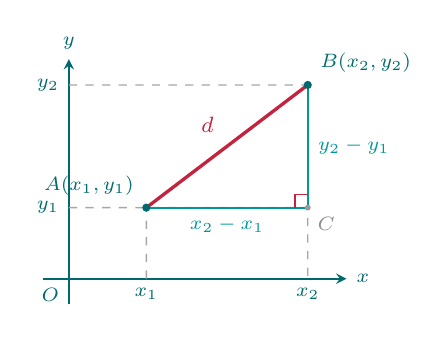
\begin{tikzpicture}[scale=0.82, >=stealth]
      \draw[->, line width=0.65pt, color=brandNavy] (-0.4,0) -- (4.3,0) node[right, font=\fontsize{7.5}{7.5}\selectfont] {$x$};
      \draw[->, line width=0.65pt, color=brandNavy] (0,-0.4) -- (0,3.4) node[above, font=\fontsize{7.5}{7.5}\selectfont] {$y$};
      \node[below left, font=\fontsize{7}{7}\selectfont, color=brandNavy] at (0,0) {$O$};
      
      \coordinate (A) at (1.2, 1.1);
      \coordinate (B) at (3.7, 3.0);
      \coordinate (C) at (3.7, 1.1);
      
      \draw[dashed, color=gray!70, line width=0.5pt] (0, 1.1) node[left, font=\fontsize{6.8}{6.8}\selectfont, color=brandNavy] {$y_1$} -- (C) -- (3.7, 0) node[below, font=\fontsize{6.8}{6.8}\selectfont, color=brandNavy] {$x_2$};
      \draw[dashed, color=gray!70, line width=0.5pt] (1.2, 0) node[below, font=\fontsize{6.8}{6.8}\selectfont, color=brandNavy] {$x_1$} -- (A);
      \draw[dashed, color=gray!70, line width=0.5pt] (0, 3.0) node[left, font=\fontsize{6.8}{6.8}\selectfont, color=brandNavy] {$y_2$} -- (B);
      
      \draw[thick, color=brandBlue] (A) -- (C) node[midway, below, font=\fontsize{7}{7}\selectfont] {$x_2 - x_1$};
      \draw[thick, color=brandBlue] (C) -- (B) node[midway, right, font=\fontsize{7}{7}\selectfont] {$y_2 - y_1$};
      \draw[very thick, color=brandCrimson] (A) -- (B) node[midway, above left=1pt, font=\fontsize{8}{8}\selectfont] {$d$};
      
      \draw[line width=0.5pt, color=brandCrimson] ($(C)+(-0.2,0)$) -- ($(C)+(-0.2,0.2)$) -- ($(C)+(0,0.2)$);
      
      \fill[brandNavy] (A) circle (1.8pt) node[above left=1pt, font=\fontsize{7.2}{7.2}\selectfont] {$A(x_1, y_1)$};
      \fill[brandNavy] (B) circle (1.8pt) node[above right=1pt, font=\fontsize{7.2}{7.2}\selectfont] {$B(x_2, y_2)$};
      \fill[gray!80] (C) circle (1.3pt) node[below right, font=\fontsize{6.8}{6.8}\selectfont, color=gray!90] {$C$};
    \end{tikzpicture}
  \end{minipage}
\end{khboxorange}

\vspace{3pt}

\begin{multicols}{2}

  % PROBLEM 1
  \noindent
  \begin{minipage}{\linewidth}
    \exhead{1} ចូរគណនាចម្ងាយរវាងពីរចំណុចដែលបានកំណត់ដោយកូអរដោនេដូចខាងក្រោម ៖
    \begin{itemize}[leftmargin=14pt, itemsep=1.2pt, topsep=1pt]
      \item[\khlabel{ក}] $A(3, 7)$ និង $B(8, -5)$
      \item[\khlabel{ខ}] $A(-1, -2)$ និង $B(3, 4)$
      \item[\khlabel{គ}] $A(9, 2)$ និង $B(6, 8)$
      \item[\khlabel{ឃ}] $A(5, -3)$ និង $B(-2, 4)$
      \item[\khlabel{ង}] $A(2, 5)$ និង $B(0, 0)$
      \item[\khlabel{ច}] $A(-6, -3)$ និង $B(2, 1)$
      \item[\khlabel{ឆ}] $A(8, 7)$ និង $B(8, -6)$
      \item[\khlabel{ជ}] $M(3, 12)$ និង $N(7, 12)$
      \item[\khlabel{ឈ}] $M(100, -203)$ និង $N(97, -200)$
      \item[\khlabel{ញ}] $D(-3, 8)$ និង $E(-4, 7)$
    \end{itemize}
  \end{minipage}

  \vspace{6pt}

  % PROBLEM 5 (REAL-LIFE APPLICATION: CITY MAP / GPS)
  \noindent
  \begin{minipage}{\linewidth}
    \exhead{5} \textbf{(អនុវត្តក្នុងជីវភាពរស់នៅ)} លើប្លង់ផែនទីទីក្រុងមួយ (គិតជា $\text{km}$) គេកំណត់ទីតាំងសំខាន់ៗ ៖ ផ្ទះតារា $H(2, 3)$ , សាលារៀន $S(8, 11)$ និងមន្ទីរពេទ្យ $M(-4, 11)$ ៖
    \begin{itemize}[leftmargin=14pt, itemsep=1.2pt, topsep=1pt]
      \item[\khlabel{ក}] គណនាចម្ងាយផ្លូវត្រង់ពីផ្ទះតារាទៅសាលារៀន ។
      \item[\khlabel{ខ}] ដ្រូនមួយហោះពីសាលារៀនទៅមន្ទីរពេទ្យ ។ គណនាចម្ងាយហោះហើររវាងទីតាំងទាំងពីរ ។
      \item[\khlabel{គ}] តើផ្ទះតារានៅជិតសាលារៀន ឬជិតមន្ទីរពេទ្យជាង ?
    \end{itemize}
  \end{minipage}

  \columnbreak

  % PROBLEM 2
  \noindent
  \begin{minipage}{\linewidth}
    \exhead{2} គេឱ្យត្រីកោណមួយដែលមានកំពូល $A(-2, 6)$ , $B(-1, -1)$ និង $C(1, 0)$ ៖
    \begin{itemize}[leftmargin=14pt, itemsep=1.2pt, topsep=1pt]
      \item[\khlabel{ក}] ចូរសង់ចំណុច $A, B$ និង $C$ នៅលើតម្រុយអ័ក្សកូអរដោនេ $xOy$ ។
      \item[\khlabel{ខ}] គណនាប្រវែងជ្រុងទាំងបីនៃត្រីកោណ $ABC$ រួចបង្ហាញថាវាជាត្រីកោណកែង ។
    \end{itemize}
    \begin{center}
      \vspace{-2pt}
      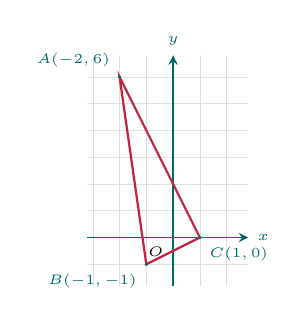
\begin{tikzpicture}[scale=0.34, >=stealth]
        \draw[very thin, gray!25, step=1] (-3.2,-1.8) grid (2.8,6.8);
        \draw[->, line width=0.5pt, color=brandNavy] (-3.2,0) -- (2.8,0) node[right, font=\fontsize{5.5}{5.5}\selectfont] {$x$};
        \draw[->, line width=0.5pt, color=brandNavy] (0,-1.8) -- (0,6.8) node[above, font=\fontsize{5.5}{5.5}\selectfont] {$y$};
        \node[below left, font=\fontsize{5}{5}\selectfont] at (0,0) {$O$};
        
        \coordinate (A) at (-2,6);
        \coordinate (B) at (-1,-1);
        \coordinate (C) at (1,0);
        
        \draw[thick, color=brandCrimson] (A) -- (B) -- (C) -- cycle;
        \fill[brandNavy] (A) circle (1.8pt) node[above left, font=\fontsize{5.5}{5.5}\selectfont] {$A(-2,6)$};
        \fill[brandNavy] (B) circle (1.8pt) node[below left, font=\fontsize{5.5}{5.5}\selectfont] {$B(-1,-1)$};
        \fill[brandNavy] (C) circle (1.8pt) node[below right, font=\fontsize{5.5}{5.5}\selectfont] {$C(1,0)$};
      \end{tikzpicture}
      \vspace{-3pt}
    \end{center}
  \end{minipage}

  \vspace{3pt}

  % PROBLEM 3
  \noindent
  \begin{minipage}{\linewidth}
    \exhead{3} ចូរបង្ហាញថាត្រីកោណ $KLM$ ដែលមានកំពូល $K(2, 8)$ , $L(10, 11)$ និង $M(5, 0)$ ជាត្រីកោណសមបាត ។
  \end{minipage}

  \vspace{4pt}

  % PROBLEM 4
  \noindent
  \begin{minipage}{\linewidth}
    \exhead{4} ចូរគណនាចម្ងាយរវាងពីរចំណុចដូចខាងក្រោម ៖
    \begin{itemize}[leftmargin=14pt, itemsep=1.2pt, topsep=1pt]
      \item[\khlabel{ក}] $A(0, 0)$ និង $B(8, -15)$
      \item[\khlabel{ខ}] $A(-2, 6)$ និង $B(3, -6)$
      \item[\khlabel{គ}] $A(-3, -5)$ និង $B(-1, -8)$
      \item[\khlabel{ឃ}] $A(5, 3)$ និង $B(11, 11)$
    \end{itemize}
  \end{minipage}

  \vspace{4pt}

  % PROBLEM 6 (REAL-LIFE APPLICATION: RADAR STATION)
  \noindent
  \begin{minipage}{\linewidth}
    \exhead{6} \textbf{(អនុវត្តជាក់ស្ដែង)} ស្ថានីយ៍រ៉ាដាមួយនៅគល់តម្រុយ $O(0, 0)$ ចាប់សញ្ញាបានក្នុងកាំ $10\text{ km}$ ។ បើកប៉ាល់មួយនៅចំណុច $P(6, 8)$ ៖ គណនាចម្ងាយ $OP$ រួចបញ្ជាក់ថាតើកប៉ាល់ស្ថិតក្នុងដែនរ៉ាដាដែរឬទេ ?
  \end{minipage}

\end{multicols}

\clearpage

% =========================================================================
% PAGE 2: SECTION 2 (កូអរដោនេនៃចំណុចកណ្ដាល)
% =========================================================================
\khsection{២}{កូអរដោនេនៃចំណុចកណ្ដាល (Coordinates of Midpoint)}

\begin{khboxorange}
  \begin{minipage}[c]{0.65\textwidth}
    \begin{itemize}[leftmargin=11pt, itemsep=1.5pt, topsep=0pt, parsep=0pt]
      \item[\color{brandNavy}\ding{228}] \textbf{គំនិតវិចារណញាណ (Feynman Intuition) ៖}\\
      ចំណុចកណ្ដាល $M(x, y)$ នៃអង្កត់ $[AB]$ គឺជា \textbf{តម្លៃមធ្យមភាគ (ពាក់កណ្ដាលផ្លូវ)} នៃកូអរដោនេទាំងពីរ — អាប់ស៊ីសជាមធ្យមនៃ $x_1, x_2$ ហើយអរដោនេជាមធ្យមនៃ $y_1, y_2$ ៖
      \vspace{1pt}
      \begin{itemize}[leftmargin=10pt, itemsep=1pt]
        \item លើអ័ក្ស $x'x$ ៖ $x - x_1 = x_2 - x \iff 2x = x_1 + x_2 \implies x = \dfrac{x_1 + x_2}{2}$
        \item លើអ័ក្ស $y'y$ ៖ $y - y_1 = y_2 - y \iff 2y = y_1 + y_2 \implies y = \dfrac{y_1 + y_2}{2}$
      \end{itemize}
      \item[\color{brandCrimson}\ding{228}] \textbf{រូបមន្តចំណុចកណ្ដាល ៖}
      \vspace{-2pt}
      \begin{equation*}
        \koreahl{$M\left(\frac{x_1 + x_2}{2}\;,\; \frac{y_1 + y_2}{2}\right)$}
      \end{equation*}
    \end{itemize}
  \end{minipage}\hfill
  \begin{minipage}[c]{0.33\textwidth}
    \centering
    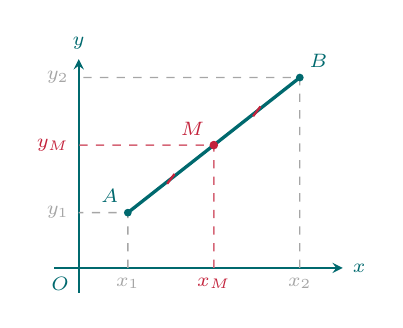
\begin{tikzpicture}[scale=0.78, >=stealth]
      \draw[->, line width=0.65pt, color=brandNavy] (-0.4,0) -- (4.3,0) node[right, font=\fontsize{7.5}{7.5}\selectfont] {$x$};
      \draw[->, line width=0.65pt, color=brandNavy] (0,-0.4) -- (0,3.4) node[above, font=\fontsize{7.5}{7.5}\selectfont] {$y$};
      \node[below left, font=\fontsize{7}{7}\selectfont, color=brandNavy] at (0,0) {$O$};
      
      \coordinate (A) at (0.8, 0.9);
      \coordinate (B) at (3.6, 3.1);
      \coordinate (M) at (2.2, 2.0);
      
      \draw[dashed, color=gray!70, line width=0.5pt] (0.8,0) node[below, font=\fontsize{6.8}{6.8}\selectfont] {$x_1$} -- (A) -- (0,0.9) node[left, font=\fontsize{6.8}{6.8}\selectfont] {$y_1$};
      \draw[dashed, color=brandCrimson!70, line width=0.5pt] (2.2,0) node[below, font=\fontsize{6.8}{6.8}\selectfont, color=brandCrimson] {$x_M$} -- (M) -- (0,2.0) node[left, font=\fontsize{6.8}{6.8}\selectfont, color=brandCrimson] {$y_M$};
      \draw[dashed, color=gray!70, line width=0.5pt] (3.6,0) node[below, font=\fontsize{6.8}{6.8}\selectfont] {$x_2$} -- (B) -- (0,3.1) node[left, font=\fontsize{6.8}{6.8}\selectfont] {$y_2$};
      
      \draw[very thick, color=brandNavy] (A) -- (B);
      
      \draw[thick, color=brandCrimson] ($(A)!0.5!(M)+(-0.06,-0.08)$) -- ($(A)!0.5!(M)+(0.06,0.08)$);
      \draw[thick, color=brandCrimson] ($(M)!0.5!(B)+(-0.06,-0.08)$) -- ($(M)!0.5!(B)+(0.06,0.08)$);
      
      \fill[brandNavy] (A) circle (1.8pt) node[above left, font=\fontsize{7}{7}\selectfont] {$A$};
      \fill[brandCrimson] (M) circle (2pt) node[above left, font=\fontsize{7.5}{7.5}\selectfont, color=brandCrimson] {$M$};
      \fill[brandNavy] (B) circle (1.8pt) node[above right, font=\fontsize{7.5}{7.5}\selectfont] {$B$};
    \end{tikzpicture}
  \end{minipage}
\end{khboxorange}

\vspace{3pt}

\begin{multicols}{2}

  % PROBLEM 1
  \noindent
  \begin{minipage}{\linewidth}
    \exhead{1} ចូរគណនាកូអរដោនេនៃចំណុចកណ្ដាលនៃអង្កត់ដែលកំណត់ដោយចំណុចទាំងពីរខាងក្រោម ៖
    \begin{itemize}[leftmargin=14pt, itemsep=1.2pt, topsep=1pt]
      \item[\khlabel{ក}] $A(4, 2)$ និង $B(6, 10)$
      \item[\khlabel{ខ}] $A(-4, -2)$ និង $B(-2, 4)$
      \item[\khlabel{គ}] $A(2, 2)$ និង $B(6, 4)$
      \item[\khlabel{ឃ}] $A(6, -3)$ និង $B(-2, -4)$
      \item[\khlabel{ង}] $A(2, 5)$ និង $B(1, 0)$
      \item[\khlabel{ច}] $A(6, -3)$ និង $B(-2, -3)$
      \item[\khlabel{ឆ}] $A(8, -2)$ និង $B(1, -5)$
      \item[\khlabel{ជ}] $M(14, 20)$ និង $B(0, -12)$
    \end{itemize}
  \end{minipage}

  \vspace{5pt}

  % PROBLEM 2
  \noindent
  \begin{minipage}{\linewidth}
    \exhead{2} ចុងទាំងពីរនៃអង្កត់ផ្ចិតរង្វង់មួយមានកូអរដោនេរៀងគ្នា $A(3, 1)$ និង $B(-2, 5)$ ៖
    \begin{itemize}[leftmargin=14pt, itemsep=1.2pt, topsep=1pt]
      \item[\khlabel{ក}] ចូរគណនាកូអរដោនេនៃផ្ចិតរង្វង់ $I$ ។
      \item[\khlabel{ខ}] ចូរគណនារង្វាស់កាំរង្វង់ រួចសង់រង្វង់នោះក្នុងប្លង់កូអរដោនេ $xOy$ ។
    \end{itemize}
    \begin{center}
      \vspace{-2pt}
      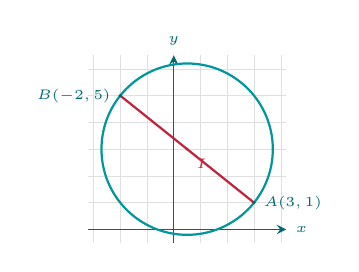
\begin{tikzpicture}[scale=0.34, >=stealth]
        \draw[very thin, gray!25, step=1] (-3.2,-0.5) grid (4.2,6.5);
        \draw[->, line width=0.5pt, color=brandNavy] (-3.2,0) -- (4.2,0) node[right, font=\fontsize{5.5}{5.5}\selectfont] {$x$};
        \draw[->, line width=0.5pt, color=brandNavy] (0,-0.5) -- (0,6.5) node[above, font=\fontsize{5.5}{5.5}\selectfont] {$y$};
        
        \coordinate (A) at (3,1);
        \coordinate (B) at (-2,5);
        \coordinate (I) at (0.5,3);
        
        \draw[thick, color=brandTeal] (I) circle (3.20);
        \draw[thick, color=brandCrimson] (A) -- (B);
        
        \fill[brandNavy] (A) circle (1.8pt) node[right, font=\fontsize{5.5}{5.5}\selectfont] {$A(3,1)$};
        \fill[brandNavy] (B) circle (1.8pt) node[left, font=\fontsize{5.5}{5.5}\selectfont] {$B(-2,5)$};
        \fill[brandCrimson] (I) circle (1.8pt) node[below right, font=\fontsize{5.5}{5.5}\selectfont] {$I$};
      \end{tikzpicture}
      \vspace{-3pt}
    \end{center}
  \end{minipage}

  \vspace{5pt}

  % PROBLEM 7 (REAL-LIFE APPLICATION: ANTENNA TOWER AT MIDPOINT)
  \noindent
  \begin{minipage}{\linewidth}
    \exhead{7} \textbf{(អនុវត្តក្នុងជីវភាពរស់នៅ)} ក្រុង $A$ និងក្រុង $B$ ស្ថិតនៅកូអរដោនេ $A(-6, 2)$ និង $B(4, 8)$ (គិតជា $\text{km}$) ។ ក្រុមហ៊ុនទូរគមនាគមន៍ចង់សង់បង្គោលអង់តែននៅចំចំណុចកណ្ដាលផ្លូវរវាងក្រុងទាំងពីរ ។ ចូរកំណត់កូអរដោនេនៃទីតាំងសង់បង្គោលអង់តែននោះ ។
  \end{minipage}

  \columnbreak

  % PROBLEM 3
  \noindent
  \begin{minipage}{\linewidth}
    \exhead{3} គេឱ្យត្រីកោណ $ABC$ ដែលមានកំពូល $A(1, 1)$ , $B(4, 1)$ និង $C(4, 4)$ ៖
    \begin{itemize}[leftmargin=14pt, itemsep=1.2pt, topsep=1pt]
      \item[\khlabel{ក}] ចូរសង់ត្រីកោណ $ABC$ លើតម្រុយអ័ក្សកូអរដោនេ $xOy$ ។
      \item[\khlabel{ខ}] គណនាប្រវែងជ្រុងទាំងបី និងបញ្ជាក់ប្រភេទត្រីកោណ $ABC$ ។
      \item[\khlabel{គ}] រកកូអរដោនេចំណុចកណ្ដាលនៃជ្រុងនីមួយៗនៃត្រីកោណ $ABC$ ។
    \end{itemize}
  \end{minipage}

  \vspace{5pt}

  % PROBLEM 4
  \noindent
  \begin{minipage}{\linewidth}
    \exhead{4} គេឱ្យ $M(1, -2)$ ជាចំណុចកណ្ដាលនៃអង្កត់ $[AB]$ ដែល $A(-2, 2)$ ។ ចូរគណនាកូអរដោនេនៃចំណុច $B$ ។
  \end{minipage}

  \vspace{5pt}

  % PROBLEM 5
  \noindent
  \begin{minipage}{\linewidth}
    \exhead{5} ត្រីកោណមួយមានកំពូល $A(2, 1)$ , $B(10, 7)$ និង $C(8, 9)$ ។ ចូរស្រាយបញ្ជាក់ថាត្រីកោណដែលផ្គុំឡើងដោយចំណុចកណ្ដាលនៃជ្រុងទាំងបីរបស់ត្រីកោណ $ABC$ ជាត្រីកោណសមបាត ។
  \end{minipage}

  \vspace{5pt}

  % PROBLEM 6
  \noindent
  \begin{minipage}{\linewidth}
    \exhead{6} ចតុកោណមួយមានកំពូល $P(-3, -2)$ , $Q(-1, 5)$ , $R(3, 1)$ និង $S(5, -4)$ ។ បើ $A, B, C$ និង $D$ ជាចំណុចកណ្ដាលរៀងគ្នានៃជ្រុង $[PQ]$ , $[QR]$ , $[RS]$ និង $[SP]$ ។ ចូរបង្ហាញថា $ABCD$ ជាប្រលេឡូក្រាម ។
  \end{minipage}

\end{multicols}

\clearpage

% =========================================================================
% PAGE 3: SECTION 3 (លំហាត់អនុវត្តន៍បន្ថែម - ភាគ ១)
% =========================================================================
\khsection{៣}{លំហាត់អនុវត្តន៍បន្ថែម (Exercises)}

\begin{multicols}{2}

  % EXERCISE 1
  \noindent
  \begin{minipage}{\linewidth}
    \exhead{1} ចូរគណនាចម្ងាយរវាងពីរចំណុចដែលមានកូអរដោនេដូចខាងក្រោម ៖
    \begin{itemize}[leftmargin=14pt, itemsep=1.5pt, topsep=1pt]
      \item[\khlabel{ក}] $(4, -2)$ និង $(8, 0)$
      \item[\khlabel{ខ}] $(-1, -4)$ និង $(0, 10)$
      \item[\khlabel{គ}] $(2, 4)$ និង $(-2, 6)$
      \item[\khlabel{ឃ}] $(-5, 0)$ និង $(6, -2)$
      \item[\khlabel{ង}] $(0, 0)$ និង $(-4, 6)$
      \item[\khlabel{ច}] $(-6, -3)$ និង $(2, 1)$
      \item[\khlabel{ឆ}] $(8, -7)$ និង $(-2, -6)$
      \item[\khlabel{ជ}] $(3, 12)$ និង $(7, 12)$
      \item[\khlabel{ឈ}] $(50, -20)$ និង $(52, -25)$
    \end{itemize}
  \end{minipage}

  \vspace{7pt}

  % EXERCISE 2
  \noindent
  \begin{minipage}{\linewidth}
    \exhead{2} ចូរគណនាកូអរដោនេនៃចំណុចកណ្ដាលនៃគូចំណុចខាងក្រោម ៖
    \begin{itemize}[leftmargin=14pt, itemsep=1.5pt, topsep=1pt]
      \item[\khlabel{ក}] $(0, 6)$ និង $(6, 12)$
      \item[\khlabel{ខ}] $(4, 2)$ និង $(-2, -4)$
      \item[\khlabel{គ}] $(-6, 0)$ និង $(-3, -1)$
      \item[\khlabel{ឃ}] $(-2, 5)$ និង $(0, 6)$
      \item[\khlabel{ង}] $(2, -3)$ និង $(-2, -5)$
      \item[\khlabel{ច}] $(-20, 5)$ និង $(12, 21)$
      \item[\khlabel{ឆ}] $(16, -8)$ និង $(-20, -32)$
      \item[\khlabel{ជ}] $(-8, 12)$ និង $(16, -14)$
      \item[\khlabel{ឈ}] $(14, 2\sqrt{2})$ និង $(4, 2\sqrt{2})$
      \item[\khlabel{ញ}] $A(3t + 5, -7)$ និង $B(t + 7, 7)$
      \item[\khlabel{ដ}] $A(a, b)$ និង $B(a, c)$
      \item[\khlabel{ឋ}] $A(2a + 5, 2b - 1)$ និង $B(4a, 9)$
    \end{itemize}
  \end{minipage}



  % EXERCISE 3
  \noindent
  \begin{minipage}{\linewidth}
    \exhead{3} ចូរគណនាប្រវែងអង្កត់ទ្រូងទាំងពីរ $[PR]$ និង $[QS]$ នៃចតុកោណ $PQRS$ ដែលមានកំពូល $P(-2, 3)$ , $Q(5, 5)$ , $R(6, -6)$ និង $S(-3, -3)$ ។
  \end{minipage}

  \vspace{6pt}

  % EXERCISE 4
  \noindent
  \begin{minipage}{\linewidth}
    \exhead{4} ចូរគណនាបរិមាត្រនៃត្រីកោណ $ABC$ ដែល $A(3, 7)$ , $B(5, 2)$ និង $C(-7, 3)$ ។ ចូរបង្ហាញថា $ABC$ ជាត្រីកោណកែង រួចគណនាផ្ទៃក្រឡារបស់វា ។
  \end{minipage}

  \vspace{6pt}

  % EXERCISE 5
  \noindent
  \begin{minipage}{\linewidth}
    \exhead{5} ចូររកតម្លៃនៃ $y$ ដើម្បីឱ្យចម្ងាយរវាងពីរចំណុច $(4, 2)$ និង $(4, y)$ ស្មើនឹង $5\text{ ឯកតា}$ ។
  \end{minipage}

  \vspace{6pt}

  % EXERCISE 6
  \noindent
  \begin{minipage}{\linewidth}
    \exhead{6} ចូររកតម្លៃនៃ $x$ ដើម្បីឱ្យចម្ងាយរវាងពីរចំណុច $(x, 6)$ និង $(-2, 5)$ ស្មើនឹង $10\text{ ឯកតា}$ ។
  \end{minipage}

  \vspace{6pt}

  % EXERCISE 7
  \noindent
  \begin{minipage}{\linewidth}
    \exhead{7} ចូររកចំណុច $C(x, 1)$ ស្ថិតក្នុងកាដ្រង់ទី ១ ($x > 0$) ដើម្បីឱ្យត្រីកោណដែលមានកំពូល $A(1, 1)$ , $B(4, 7)$ និង $C(x, 1)$ ជាត្រីកោណសមបាតដែល $AB = AC$ ។
  \end{minipage}

  \vspace{6pt}

  % EXERCISE 8
  \noindent
  \begin{minipage}{\linewidth}
    \exhead{8} កំពូលនៃត្រីកោណមួយមានកូអរដោនេ $A(-3, 2)$ , $B(9, 2)$ និង $C(3, 10)$ ៖
    \begin{itemize}[leftmargin=14pt, itemsep=1.5pt, topsep=1pt]
      \item[\khlabel{ក}] ចូរគណនាប្រវែងជ្រុងទាំងបីនៃត្រីកោណ ។
      \item[\khlabel{ខ}] ចូរប្រាប់ប្រភេទនៃត្រីកោណនោះ ។
    \end{itemize}
  \end{minipage}

  \vspace{6pt}

  % EXERCISE 9
  \noindent
  \begin{minipage}{\linewidth}
    \exhead{9} កំពូលនៃចតុកោណមួយមានកូអរដោនេ $A(-1, -2)$ , $B(5, -2)$ , $C(5, 4)$ និង $D(-1, 4)$ ៖
    \begin{itemize}[leftmargin=14pt, itemsep=1.5pt, topsep=1pt]
      \item[\khlabel{ក}] ចូរគណនាប្រវែងជ្រុង និងប្រវែងអង្កត់ទ្រូងនៃចតុកោណ ។
      \item[\khlabel{ខ}] តើគេសន្និដ្ឋានដូចម្ដេចចំពោះចតុកោណនេះ ?
    \end{itemize}
  \end{minipage}

  \vspace{6pt}

  % EXERCISE 10
  \noindent
  \begin{minipage}{\linewidth}
    \exhead{10} កូអរដោនេកំពូលរបស់ចតុកោណមួយមាន $A(2, -1)$ , $B(6, 4)$ , $C(2, 9)$ និង $D(-2, 4)$ ៖
    \begin{itemize}[leftmargin=14pt, itemsep=1pt, topsep=1pt]
      \item[\khlabel{ក}] គណនាប្រវែងជ្រុង និងប្រវែងអង្កត់ទ្រូងនៃចតុកោណ ។
      \item[\khlabel{ខ}] ចូរប្រាប់ប្រភេទនៃចតុកោណនេះ ។
    \end{itemize}
    \begin{center}
      \vspace{-3pt}
      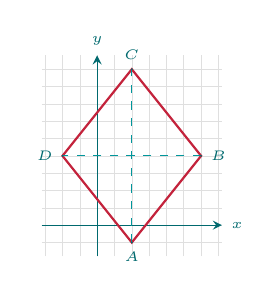
\begin{tikzpicture}[scale=0.22, >=stealth]
        \draw[very thin, gray!25, step=1] (-3.2,-1.8) grid (7.2,9.8);
        \draw[->, line width=0.45pt, color=brandNavy] (-3.2,0) -- (7.2,0) node[right, font=\fontsize{4.5}{4.5}\selectfont] {$x$};
        \draw[->, line width=0.45pt, color=brandNavy] (0,-1.8) -- (0,9.8) node[above, font=\fontsize{4.5}{4.5}\selectfont] {$y$};
        
        \coordinate (A) at (2,-1);
        \coordinate (B) at (6,4);
        \coordinate (C) at (2,9);
        \coordinate (D) at (-2,4);
        
        \draw[thick, color=brandCrimson] (A) -- (B) -- (C) -- (D) -- cycle;
        \draw[dashed, color=brandBlue, line width=0.4pt] (A) -- (C);
        \draw[dashed, color=brandBlue, line width=0.4pt] (B) -- (D);
        
        \fill[brandNavy] (A) circle (1.6pt) node[below, font=\fontsize{4.8}{4.8}\selectfont] {$A$};
        \fill[brandNavy] (B) circle (1.6pt) node[right, font=\fontsize{4.8}{4.8}\selectfont] {$B$};
        \fill[brandNavy] (C) circle (1.6pt) node[above, font=\fontsize{4.8}{4.8}\selectfont] {$C$};
        \fill[brandNavy] (D) circle (1.6pt) node[left, font=\fontsize{4.8}{4.8}\selectfont] {$D$};
      \end{tikzpicture}
      \vspace{-3pt}
    \end{center}
  \end{minipage}

  \vspace{5pt}

  % EXERCISE 11
  \noindent
  \begin{minipage}{\linewidth}
    \exhead{11} ចតុកោណមួយមានកំពូល $A(-2, -3)$ , $B(-3, 1)$ , $C(5, -1)$ និង $D(4, -3)$ ។ តើចតុកោណនេះមានរាងជាអ្វី ? ចូរស្រាយបញ្ជាក់ ។
  \end{minipage}

  \vspace{5pt}

  % EXERCISE 12
  \noindent
  \begin{minipage}{\linewidth}
    \exhead{12} ចូរគណនាកូអរដោនេនៃចំណុចកណ្ដាលនៃ $[AB]$ រួចដៅចំណុចក្នុងតម្រុយអរតូណរមេតាមករណីនីមួយៗ ៖
    \begin{itemize}[leftmargin=14pt, itemsep=1.5pt, topsep=1pt]
      \item[\khlabel{ក}] $A(5, 8)$ និង $B(5, 12)$
      \item[\khlabel{ខ}] $A(-5, 2)$ និង $B(-5, 14)$
    \end{itemize}
  \end{minipage}

  \vspace{5pt}

  % EXERCISE 13
  \noindent
  \begin{minipage}{\linewidth}
    \exhead{13} ចូរគណនាកូអរដោនេនៃចំណុចកណ្ដាល $M$ នៃអង្កត់រវាងពីរចំណុច $A(-3, -1)$ និង $B(5, 7)$ ។ ចូរគណនាប្រវែង $AM$ និង $BM$ រួចផ្ទៀងផ្ទាត់ថា $AM = BM$ ។
  \end{minipage}

  \vspace{5pt}

  % EXERCISE 14
  \noindent
  \begin{minipage}{\linewidth}
    \exhead{14} គេឱ្យ $M(1, -2)$ ជាចំណុចកណ្ដាលនៃអង្កត់ $[AB]$ ដែល $A(-2, 2)$ ។ ចូរគណនាកូអរដោនេនៃចំណុច $B$ ។
  \end{minipage}

  \vspace{5pt}

  % EXERCISE 15
  \noindent
  \begin{minipage}{\linewidth}
    \exhead{15} គេឱ្យ $M(4, -4)$ ជាចំណុចកណ្ដាលនៃអង្កត់ $[AB]$ ដែល $B(0, 6)$ ។ ចូរគណនាកូអរដោនេនៃចំណុច $A$ ។
  \end{minipage}

  \vspace{5pt}

  % EXERCISE 16
  \noindent
  \begin{minipage}{\linewidth}
    \exhead{16} រង្វង់មួយមានផ្ចិត $F(-2, 6)$ ។ អង្កត់ផ្ចិតរង្វង់នេះមានចំណុចចុងមួយត្រង់ $V(3, 8)$ ។ គណនាកូអរដោនេនៃចំណុច $T$ ដែលជាចំណុចម្ខាងទៀតនៃអង្កត់ផ្ចិត $[TV]$ រួចសង់រង្វង់នេះលើប្លង់កូអរដោនេ ។
  \end{minipage}

  \vspace{5pt}

  % EXERCISE 17
  \noindent
  \begin{minipage}{\linewidth}
    \exhead{17} ចតុកោណមួយមានកំពូល $E(5, 3)$ , $F(5, -5)$ , $G(-3, -3)$ និង $H(-1, 5)$ ។ ចូរគណនាកូអរដោនេចំណុចកណ្ដាល $A, B, C$ និង $D$ នៃជ្រុង $[EF]$ , $[FG]$ , $[GH]$ និង $[EH]$ រៀងគ្នា ។ តើចតុកោណ $ABCD$ មានរាងជាអ្វី ?
  \end{minipage}

  \columnbreak

  % EXERCISE 18
  \noindent
  \begin{minipage}{\linewidth}
    \exhead{18} ចតុកោណកែងមួយកំណត់ដោយចំណុច $A(3, 2)$ , $B(9, 2)$ , $C(9, 6)$ និង $D(3, 6)$ ។ ចូរស្រាយបញ្ជាក់ថា ចតុកោណដែលកំណត់ដោយចំណុចកណ្ដាលនៃជ្រុងទាំងបួនរបស់ចតុកោណកែងខាងលើជាចតុកោណស្មើ (រ៉ុម) ។
    \begin{center}
      \vspace{-2pt}
      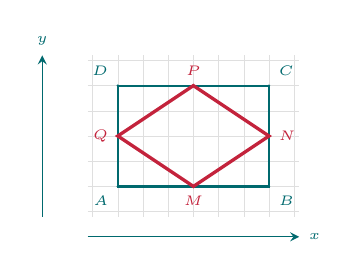
\begin{tikzpicture}[scale=0.32, >=stealth]
        \draw[very thin, gray!25, step=1] (1.8,0.8) grid (10.2,7.2);
        \draw[->, line width=0.45pt, color=brandNavy] (1.8,0) -- (10.2,0) node[right, font=\fontsize{4.8}{4.8}\selectfont] {$x$};
        \draw[->, line width=0.45pt, color=brandNavy] (0,0.8) -- (0,7.2) node[above, font=\fontsize{4.8}{4.8}\selectfont] {$y$};
        
        \coordinate (A) at (3,2);
        \coordinate (B) at (9,2);
        \coordinate (C) at (9,6);
        \coordinate (D) at (3,6);
        
        \coordinate (M1) at (6,2);
        \coordinate (M2) at (9,4);
        \coordinate (M3) at (6,6);
        \coordinate (M4) at (3,4);
        
        \draw[thick, color=brandNavy] (A) -- (B) -- (C) -- (D) -- cycle;
        \draw[very thick, color=brandCrimson] (M1) -- (M2) -- (M3) -- (M4) -- cycle;
        
        \fill[brandNavy] (A) circle (1.5pt) node[below left, font=\fontsize{4.5}{4.5}\selectfont] {$A$};
        \fill[brandNavy] (B) circle (1.5pt) node[below right, font=\fontsize{4.5}{4.5}\selectfont] {$B$};
        \fill[brandNavy] (C) circle (1.5pt) node[above right, font=\fontsize{4.5}{4.5}\selectfont] {$C$};
        \fill[brandNavy] (D) circle (1.5pt) node[above left, font=\fontsize{4.5}{4.5}\selectfont] {$D$};
        
        \fill[brandCrimson] (M1) circle (1.5pt) node[below, font=\fontsize{4.5}{4.5}\selectfont, color=brandCrimson] {$M$};
        \fill[brandCrimson] (M2) circle (1.5pt) node[right, font=\fontsize{4.5}{4.5}\selectfont, color=brandCrimson] {$N$};
        \fill[brandCrimson] (M3) circle (1.5pt) node[above, font=\fontsize{4.5}{4.5}\selectfont, color=brandCrimson] {$P$};
        \fill[brandCrimson] (M4) circle (1.5pt) node[left, font=\fontsize{4.5}{4.5}\selectfont, color=brandCrimson] {$Q$};
      \end{tikzpicture}
      \vspace{-3pt}
    \end{center}
  \end{minipage}

  \vspace{6pt}

  % EXERCISE 19
  \noindent
  \begin{minipage}{\linewidth}
    \exhead{19} គេឱ្យរង្វង់ $(S)$ មួយមានអង្កត់ផ្ចិត $[AB]$ ដែល $A(-4, 5)$ និង $B(2, -3)$ ៖
    \begin{itemize}[leftmargin=14pt, itemsep=1.5pt, topsep=1pt]
      \item[\khlabel{ក}] ចូរកំណត់កូអរដោនេផ្ចិត $I$ របស់រង្វង់ $(S)$ ។
      \item[\khlabel{ខ}] គណនារង្វាស់កាំនៃរង្វង់ $(S)$ ។
      \item[\khlabel{គ}] ចូរស្រាយបញ្ជាក់ថា ចំណុច $M(2, 5)$ និង $N(-5, 4)$ ស្ថិតនៅលើរង្វង់ $(S)$ ។
    \end{itemize}
  \end{minipage}

  \vspace{6pt}

  % EXERCISE 20
  \noindent
  \begin{minipage}{\linewidth}
    \exhead{20} គេមានអង្កត់ $[P_1 P_2]$ ដែល $P_1(x_1, y_1)$ និង $P_2(x_2, y_2)$ ។ គណនាកូអរដោនេនៃចំណុច $A$ និង $B$ ដែលចែកអង្កត់ $[P_1 P_2]$ ជាបីផ្នែកស្មើៗគ្នា ($P_1 A = AB = B P_2$) ។
  \end{minipage}

  \vspace{6pt}

  % EXERCISE 21
  \noindent
  \begin{minipage}{\linewidth}
    \exhead{21} គេមានចំណុច $P_1(x_1, y_1)$ , $P_m\left(\dfrac{x_1 + x_2}{2}\;,\; \dfrac{y_1 + y_2}{2}\right)$ និង $P_2(x_2, y_2)$ ។\\
    ចូរបង្ហាញថា $P_1 P_m + P_m P_2 = P_1 P_2$ ។
  \end{minipage}

  \vspace{6pt}

  % EXERCISE 22
  \noindent
  \begin{minipage}{\linewidth}
    \exhead{22} គេឱ្យ $A(1, 0)$ និង $B(3, 2)$ រួចសង់រង្វង់ដែលមានអង្កត់ផ្ចិត $AB$ ៖
    \begin{itemize}[leftmargin=14pt, itemsep=1.5pt, topsep=1pt]
      \item[\khlabel{ក}] ចូររកកូអរដោនេនៃផ្ចិតរង្វង់ដែលតាងដោយចំណុច $I$ ។
      \item[\khlabel{ខ}] $M$ ជាចំណុចមួយដែលមានកូអរដោនេ $M\left(\dfrac{5}{2}\;,\; y\right)$ ។ ចូរកំណត់តម្លៃនៃ $y$ ដើម្បីឱ្យ $M$ ស្ថិតនៅលើរង្វង់ រួចបញ្ជាក់ថាតើមានចំណុច $M$ ប៉ុន្មានទីតាំង ?
    \end{itemize}
  \end{minipage}

  \vspace{6pt}

  % EXERCISE 23
  \noindent
  \begin{minipage}{\linewidth}
    \exhead{23} គេឱ្យបីចំណុច $A(x, 1)$ , $B(5, y)$ និង $C(x + 3, 5)$ ។ ចូរកំណត់តម្លៃនៃ $x$ និង $y$ ដើម្បីឱ្យត្រីកោណ $ABC$ ជាត្រីកោណកែងសមបាតកំពូល $A$ ។
  \end{minipage}

\end{multicols}

\end{document}
